
% TODO: do we need to define the word "distribution?!"

\chapter{KDEs and distributions}
\label{ch:KDEs}

\index{histogram}
\section{Limitations of histograms}

Histograms are a great tool for seeing the distribution of a numerical,
univariate sample. As we'll see in this chapter, though, they have some
deficiencies. One problem is that a data set doesn't uniquely determine a
histogram: instead, we must specify parameters such as the bin size and the
``alignment'' of the bins (\textit{i.e.}, where exactly the breaks occur), and
the resulting display is colored (no pun intended) by those choices.

Consider this simple data set\footnote{From Janert, P. K. (2010). Data Analysis
with Open Source Tools: A Hands-On Guide for Programmers and Data Scientists (1
edition). O'Reilly Media.}:

\begin{center}
\texttt{2.1, 2.3, 1.9, 1.8, 1.4, 2.6, 1.7, 2.2}
\end{center}

Suppose we choose a bin width of 1. If we positioned the \textit{left} edge of
each bin at 0, 1, 2, 3, ..., we would get the histogram on the left side of
Figure~\ref{fig:histBinParadox}.

\begin{Verbatim}[fontsize=\footnotesize,samepage=true,frame=single]
data = np.array([2.1, 2.3, 1.9, 1.8, 1.4, 2.6, 1.7, 2.2])
plt.hist(data, bins=[0,1,2,3,4])
\end{Verbatim}

Our interpretation would probably be: ``looks like the values occur pretty
uniformly throughout the range 1-3.''

But if we shifted our bin alignment to be on the ``halves'' (0.5, 1.5, 2.5,
...), we get this histogram on the \textit{right} side of
Figure~\ref{fig:histBinParadox}.

\begin{Verbatim}[fontsize=\footnotesize,samepage=true,frame=single]
plt.hist(data, bins=[-.5,0.5,1.5,2.5,3.5,4.5])
\end{Verbatim}

Now we may be liable to think: ``it looks like a steeply-peaked distribution
with most values right near the center value of 2.''

\smallskip
Yet the data is the \textit{same}! :-O

\begin{figure}[ht]
\centering
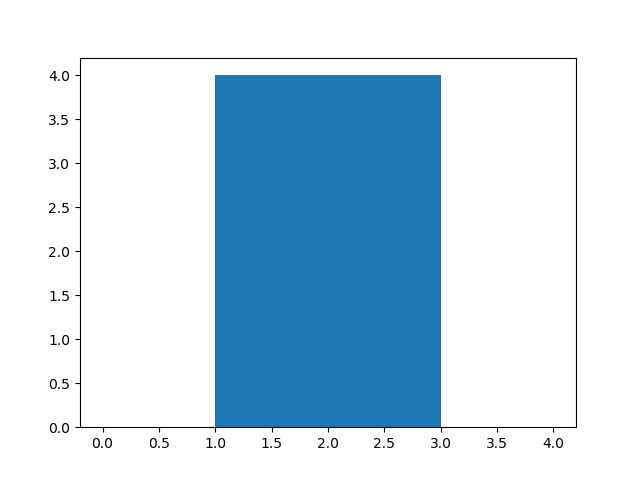
\includegraphics[width=0.45\textwidth]{hist1.png}
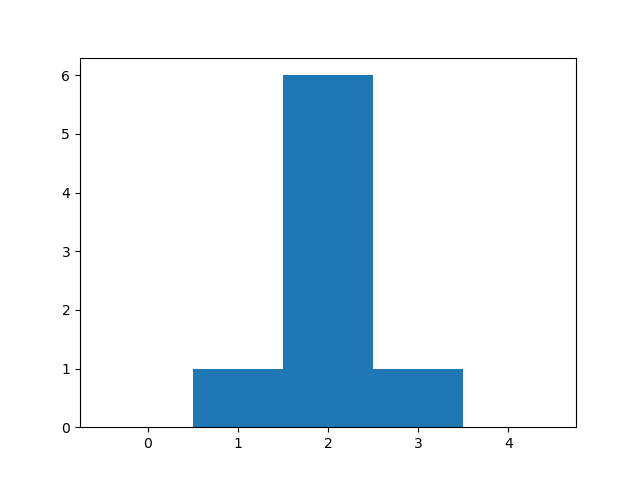
\includegraphics[width=0.45\textwidth]{hist2.png}
\caption{Two histograms of the \textit{same} data set!}
\label{fig:histBinParadox}
\end{figure}
\begin{center}
\end{center}
\vspace{-.6in}

\subsection{Data vs.~process}

Now you might dismiss this idiosyncrasy as merely a one-off quirk that only
shows up when the data is carefully arranged so as to trigger it. And there's
some truth to that. But the real problem with histograms is bigger and more
conceptual: it has to do with \textit{what we're really trying to visualize in
the first place.}

\index{data-generating process (DGP)}

In Data Science, paradoxically, very often we don't actually care about the
\textit{data} so much as we care about the underlying \textit{process} that
generated the data. This ``Data-Generating Process'' (DGP) -- whether it's a
geographic fault, a mystery author, a sports team, or an economy -- leaves
behind evidence of its behavior (seismic tremors, sentences, sports statistics,
income levels) which we dutifully collect and then analyze. The purpose is
(almost) always to draw inferences about how that DGP works, not to learn about
the individual bread crumbs themselves.

To our present point, when we look at a histogram of (say) GPAs of a sample of
UMW students, we're not actually interested in what those sampled GPAs
precisely are, strange as that may sound. We're instead interested in what they
tell us about UMW student GPAs in general. We want to draw conclusions about
the \textbf{population} by looking at the \textbf{sample}.\footnote{If you
haven't encountered these words before, the ``population'' is the entire set of
relevant objects of study that are out there in the world, most of which we'll
never get a direct measurement for because they're just too numerous. The
``sample'' is the small subset of the population that we did get a measurement
for. A classic example is political polling: we don't really care that much how
the 2,000 people in our telephone poll are going to vote for President; what we
care about is how the country as a whole will vote for President. So we assume
that the sample is reflective of the population, and reason accordingly using
statistical tests as our guide.}

Let's say we hung out at the fountain on campus walk, and asked unsuspecting
volunteers to let us measure how tall they were. The histogram of the result
might look like Figure~\ref{kdehist}.

\begin{figure}[ht]
\centering
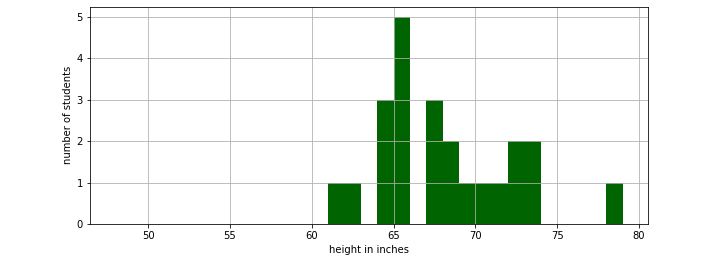
\includegraphics[width=0.7\textwidth]{kdehist.png}
\caption{A histogram of a sample of UMW student heights.}
\label{kdehist}
\end{figure} 

The histogram is using ``1 inch'' as a bin size. By inspecting it, we can see
that the shortest person in our sample was 62 inches tall (or 5-foot-2), the
tallest was 78 inches (6-foot-6), and the most common height was 65 inches
(5-foot-5), among other things.

But consider this. Our sample had five students who were 5-foot-5, three who
were 5-foot-7, but \textit{none} who were 5-foot-6. This is perfectly possible
with samples, of course -- you're only getting a random set of students, and
there are bound to be little quirks like this. But on what basis do we label it
a ``quirk?''

If you're like me, your inclination is to say, ``yeah, okay, in this particular
sample we happened to be missing any 5-foot-6 people, but it's not like we're
going to draw any grand conclusions from that fact. We're not going to deduce
that `UMW students are almost never 5-foot-6 -- they're almost always either a
tad shorter or a tad taller than that.' Such a conclusion would be ludicrous!''

\index{background knowledge}

I sympathize and agree. But really, we only know this because we bring
\textbf{background knowledge} to the problem. We've all seen lots of people of
various heights, and we know something about how genetics and nutrition and
other factors play into a person's height, and it just screams ``wrong!'' to
think that there's some magic ``missing height'' out there, right in the middle
of otherwise quite common heights, that for some reason is virtually
unattainable.

Think about it, though: if we were studying an \textit{unknown} phenomenon,
about which we had no previous experience, it would be pretty audacious for us
to infer the existence of lots of ``66's'' which we never actually observed,
simply on the grounds that there were lots of 65's and 67's in our sample. My
point is not to forsake your background knowledge: quite the opposite, you
should make good use of it! My point is only to draw attention to the
justification we're using to infer the existence of plenty of 66-inch-tall
(5-foot-6) people in the population, even though we never actually observed
any.

So my main point is this. Although we look at a histogram like this one in
order to see ``the lay of the land'' -- to see which values of the numeric
variable are more frequent, and which are less frequent -- if we're smart we
can't help but recognize two different aspects to the figure. Some of the
histogram's features are generalizable, and indicative of what the population
probably looks like: we'd (correctly) gather that many or most UMW students
were between 60 and 80 inches tall, with the majority in the 65-ish to 75-ish
range. But some of its features we'd (correctly) characterize as mere artifacts
of this particular sample, like the weird fact that we happen to have several
65-inchers and 67-inchers but no 66-inchers.

What we'd really like is a plot that obscures (or ``smooths over'') the second
kind of thing, while still revealing the first kind of thing. In other words,
we'd like a plot that shows us the features of the data that are probably
generalizable, while hiding the individual nooks and crannies. Such a plot is
coming right up in Section~\ref{kdes}, below.

Just to finish venting, I'll list yet another couple of problems with
histograms:

\begin{itemize}
\itemsep.1em
\item They inherently lose information, since by definition data points with
specific, precise values are munged into ``the nearest bin.''
\item They don't handle outliers very well. A single outlier way outside the
normal range forces us to either (a) include a lot of empty cells in the
middle, or (b) choose an unreasonably wide bin width that doesn't work for the
majority of points.
\end{itemize}

\section{Kernel Density Estimates (KDEs)}

\label{kdes}

One solution to these unfortunate histogram problems is a more advanced
technique called a \textbf{Kernel Density Estimate}, or a \textbf{KDE}.

\index{kernel}
\index{Gaussian (kernel)}
\index{normal distribution}
\label{Gaussian}

A ``kernel'' is defined as a single, strongly-peaked function that has an area
under its curve of exactly 1. Normally (no pun intended!) we will use a
\textit{Gaussian kernel}, which means ``a bell curve a la the normal
distribution'':

\begin{center}
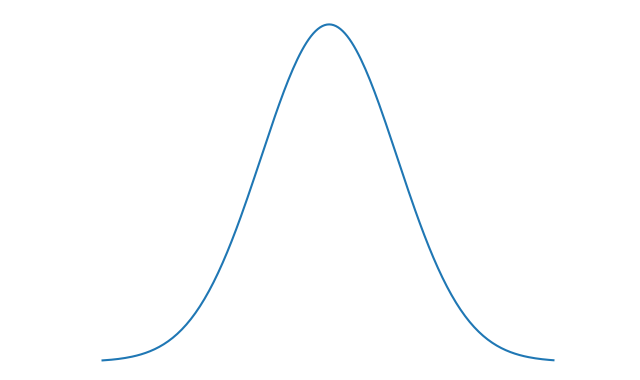
\includegraphics[width=0.4\textwidth]{lilGaussian.png}
\end{center}

(In math and stats, ``Gaussian'' and ``normal'' are synonyms.)

\index{bandwidth}
\index{standard deviation}

One thing we have to decide on is the \textit{width} of this kernel --- which
in our case essentially means ``the standard deviation of the normal
distribution we're using.'' This is kind of like having to choose the bin width
for histograms, but in practice the choice turns out not to be as critical. The
width we choose is called the kernel's \textbf{bandwidth}.

Okay, now visualize this. In order to form a KDE, we place a \textit{copy} of
this kernel on the x-axis at each data point, and then add up all the kernel
contributions to make a smooth curve. This has the effect of smoothing out all
the jaggedy ups and downs of the actual histogram. The goal is to reflect the
``true, underlying'' shape of the data for the entire population.

\index{gaussian\_kde@\texttt{gaussian\_kde()} (SciPy)}
\index{kdeplot@\texttt{kdeplot()} (Seaborn)}

There are several different ways to do this with Python packages. The Seaborn
library has a good ``\texttt{kdeplot()}'' function. Using straight SciPy, we
can call the \texttt{gaussian\_kde()} function and pass it the bandwidth as a
second argument. This returns a function that can be used to evaluate the KDE
at any data point. (Read that sentence again: a function that returns a
function? It can be confusing.) Then, we can plot it by creating a range of
values to evaluate the KDE at, and plotting those values against the KDE's
values.

It's easier than it sounds when you run the actual code:

\index{bw\_method@\texttt{bw\_method} (for \texttt{gaussian\_kde()})}

\begin{Verbatim}[fontsize=\footnotesize,samepage=true,frame=single]
import scipy.stats
kde = scipy.stats.gaussian_kde(data,bw_method=.5)
x_vals = np.arange(0,10,.1)
plt.plot(x_vals,kde(x_vals))
\end{Verbatim}

\index{bandwidth}

The ``\texttt{data}'' argument to \texttt{gaussian\_kde()} is the array you're
working with, and ``\texttt{bw\_method}'' (a dumb name) gives the kernel's
bandwidth. (\texttt{x\_vals} is an array of the x coordinates you want to plot
the KDE for, and should cover the range.)

Now stare at the four plots in Figure~\ref{kdesfig}. These are all KDEs for
the green Figure~\ref{kdehist} histogram, but each one uses a different
bandwidth. Choosing a larger kernel bandwidth effectively smooths out the KDE
more, spreading the contribution of each point quite a bit farther from its
original position. Choosing a narrower kernel focuses each data point's
contribution more precisely at its actual value, making the plot choppier.

\begin{figure}[ht]
\centering
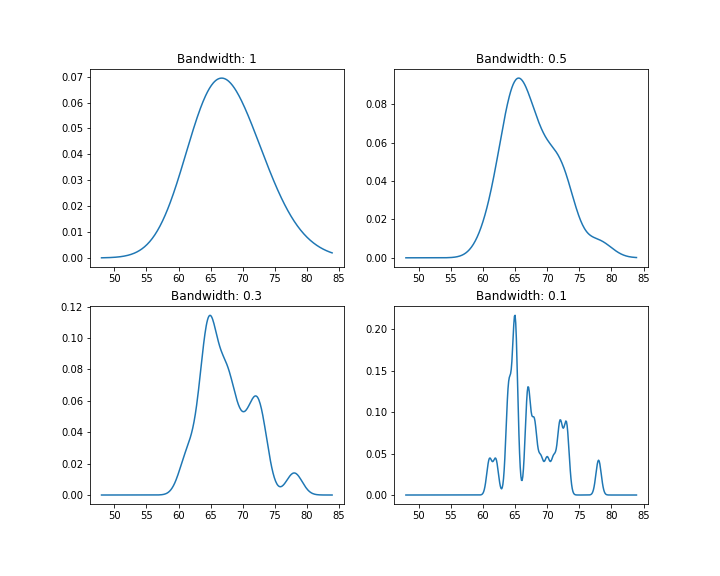
\includegraphics[width=1\textwidth]{kdes.png}
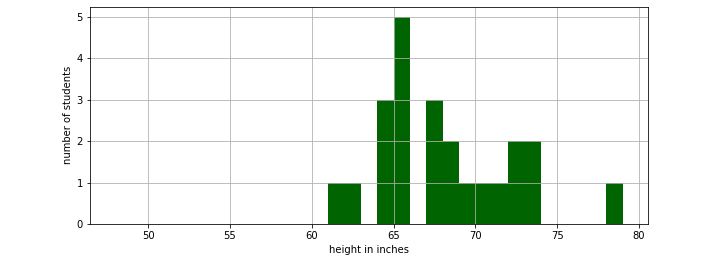
\includegraphics[width=0.7\textwidth]{kdehist.png}
\caption{Gaussian KDEs with bandwidths of 1, .5, .3, and .1, respectively, for
the data behind the green Figure~\ref{kdehist} histogram (repeated here).}
\label{kdesfig}
\end{figure}

In practice, it's another parameter to play with. If the data follows a smooth
distribution, you can use a wider bandwidth which will ``blur'' each data point
more and give a more intuitive view of the general distribution
characteristics. If the distribution is more wiggly, though, you need a
narrower bandwidth to see all the relevant detail. Which of the
Figure~\ref{kdesfig} bandwidths do you think best captures the ``true''
distribution of the points in the histogram?

Like most things in Data Science (and in life), there's no one true
hard-and-fast right answer. There is instead a range of points of view, many
of which may be illuminating.
